\chapter{Reconnaissance automatique des émotions}
\label{chapitre3}
«Si vous voulez être libre de vos émotions il faut avoir la connaissance réelle, immédiate de vos émotions.»  (Arnaud Desjardins, 1925-2011)


\section{Les architectures de couches neuronales utilisées dans le traitement de la parole}
\textcolor{red}{peut etre remonter cette partie dans le deuxieme chapitre?}

Dans le cadre de cette thèse, nous travaillons sur les informations contenues dans la parole. L'utilisation du MLP n'est plus la plus performante des approches pour représenter les données de type parole. Il existe d'autres architectures de couches neuronales bien plus compatibles avec ces données. En effet, le principe inconvénient du MLP, c'est que les données sont considérées une à une, il est donc difficile de gérer les relations temporelles par exemple.Le passé et le futur n'influence pas directement les systèmes d'apprentissage. Une entrée est donc considérée seule et sans contexte.

Or nous savons que la parole est caractérisée par l'entièreté de sa séquence. Si nous faisons un parallèle avec un texte, une lettre seule ne veut rien dire. Accompagnée d'autres lettres, elles forment un mot. Ces mots sont eux-mêmes agencés avec d'autres mots pour donnr un sens à une phrase.

Comme la parole est dépendante des états précédents, il est nécessaire d'utiliser des réseaux permettant de prendre en compte les états précédents voir les états suivants. Dans cette section, nous allons décrire des architectures neuronales permettant de conserver l'historique des états précédents, qui sont par conséquent utilisées dans le traitement de la parole.

\subsection{Réseaux neuronaux convolutifs}
Les réseaux neuronaux convolutifs (Convolutional Neural Network en anglais), abrégé CNN~\cite{LeCun1989} sont prépondérant dans l'analyse d'image. L'une des premières tâches mettant en œuvre des réseaux convolutifs a été la reconnaissance d'écriture manuscrite~\cite{LeCun1998}, notant de chiffres et de nombres. En effet ils traitent des données représentées en deux dimensions comme des images (disposition des pixel en 2D), permettant des résultats probants sur les tâches de reconnaissance d'objets au sein d'une image~\cite{Traore2018}, ou la reconnaissance de visages~\cite{Liu2016}. Ils sont également utilisés en parole, lorsque l'on considère le signal comme un spectrogramme par exemple~\cite{Abdel2014}. Récemment, cette architecture a été utilisée pour répondre à des tâches concernant la reconnaissance d'émotion, aussi bien à partir d'images~\cite{Pitaloka2017,Mehendale2020} qu'à partir d'audio~\cite{Zhang2016}.

\begin{figure}[h]
  \centering
  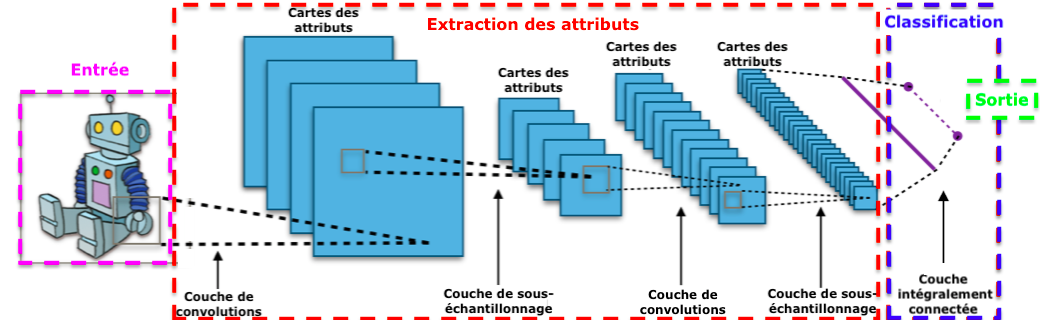
\includegraphics[width=14cm]{./Chapitre3/figures/cnn.png}
  \caption{Représentation schématique du traitement d'une image par un réseau de type convolutionnel. Image provenant de Wikipedia.}
  \label{fig:cnn}
\end{figure}


Comme son nom l'indique, ce réseau effectue des produits de convolutions en fonction de la configuration de son champ récepteur. Il se décompose en trois opérations : la convolution, le pooling puis l'activation de type ReLu.
Si nous revenons dans le détail, ils ont été conçus pour des données présentées sous forme de tableaux de N dimensions. Comme nous l'avons vu précédemment, ils sont pertinents dans le traitement des images, puisque ces dernières se représentent sous la forme d'une addition de tableaux de 2D (trois pour des images RGB, quatre si on considère la transparence de l'image, un seul pour une image en noir et blanc).

On peut décrire le fonctionnement d'un réseau convolutif par une succession d'étapes :

\begin{itemize}
  \item l'étape de convolution consiste à faire glisser un filtre de taille k sur l'ensemble du tableau et à calculer le produit de la convolution entre chaque fenêtre de taille k et le filtre. Le procédé est schématisé dans la figure~\ref{fig:cnn}.
  \item l'étape de sous-échantillonnage (pooling en anglais) va permettre de réduire la taille totale du tableau tout en conservant les informations pertinentes pour le système, comme expliqué dans la figure~\ref{fig:cnn}. Différentes méthodes de sous-échantillonnage existent mais les plus usités sont les fonctions mathématiques de type minimum, maximum ou moyenne du tableau. Cette étape est importante, puisqu'elle permet de garantir une réduction du nombre de paramètres, qui peut augmenter très rapidement avec les couches de convolution.
  \item optionnellement, on peut ajouter des étapes de correction. Ces couches ont pour rôle de faciliter la prise de décision au sein du réseau, en activant ou désactivant certaines connexions entre les différents neurones. Elles se présentent sous la forme de fonctions mathématiques qui vont être appliquées en sortie d'une couche. Principalement on retrouve la fonction ReLU, la tangente hyperbolique et la fonction sigmoïde.
\end{itemize}

Il y a donc deux hyper-paramètres spécifiques à considérer lors de la construction d'un réseau convolutif : le nombre de noyaux de convolution, qui va déterminer la taille du filtre et le pas qui va contrôler les chevauchements entre les champs récepteurs. Ces deux variables permettent de calculer la taille de la sortie.

\subsection{Réseaux Neuronaux Récurrents}
\begin{figure}[h]
  \centering
  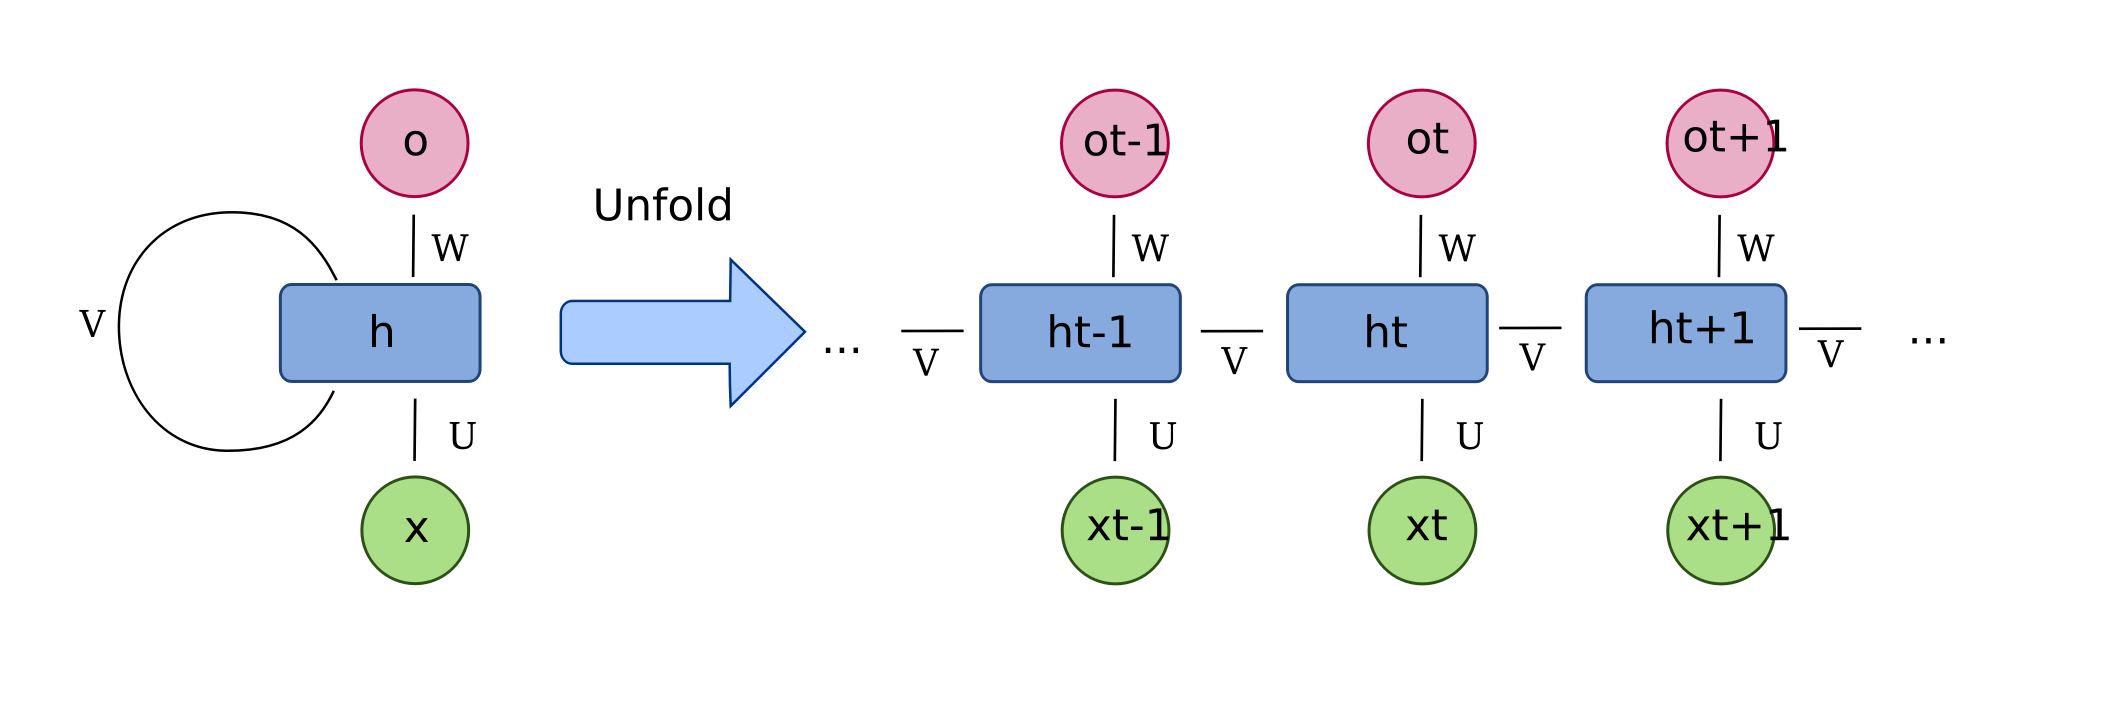
\includegraphics[width=14cm]{./Chapitre3/figures/rnn.png}
  \caption{Représentation schématique d'un réseau neuronal récurrent. La partie gauche correspond à une récurrence sur une couche entière $h$. La partie droite explicite la récurrence au niveau de la couche $h$. Image provenant de Wikipedia.}
  \label{fig:rnn}
\end{figure}


Les réseaux neuronaux récurrents (RNN)~\cite{Jordan1986} décrivent une architecture neuronale qui est encore très utilisée de nos jours pour résoudre de nombreuses tâches. En effet, ils permettent de modéliser des séquences dont la taille est variable, en présentant toute la séquence dans l'ordre au système. Il est donc possible de faire correspondre plusieurs entrées à plusieurs sorties (appelé \textit{many-to-many}) ainsi que plusieurs entrées à une seule sortie (appelé \textit{many-to-one}) contrairement aux réseaux neuronaux classiques, permettant uniquement de faire correspondre une entrée à une sortie (appelé \textit{one-to-one}).

Ils permettent également de prendre en compte l'aspect chronologique de la séquence et met en avant les dépendances temporelles dans les séquences.
Pour ajouter cet aspect mémoriel, une deuxième entrée est ajoutée au neurone, correspondant à la sortie précédente, comme explicité dans le schéma~\ref{fig:rnn}. Cette boucle va donc permettre de conserver des informations entre les différentes itérations du système.

Même si en théorie leur mémoire devrait pouvoir contenir tous les éléments de la séquence visualisée, ce n'est pas le cas dans les faits. Bengio et al.~\cite{Bengio1994} ont montré que ces systèmes ont beaucoup de mal à modéliser des dépendances éloignées. On pourra difficilement modéliser une dépendance entre un début de conversation et sa fin si la séquence est trop longue par exemple.

C'est pour palier à ce problème qu'un autre type de réseau récurrent a vu le jour.

\subsection{Réseaux récurrents à mémoire court et long terme}
\begin{figure}[h]
  \centering
  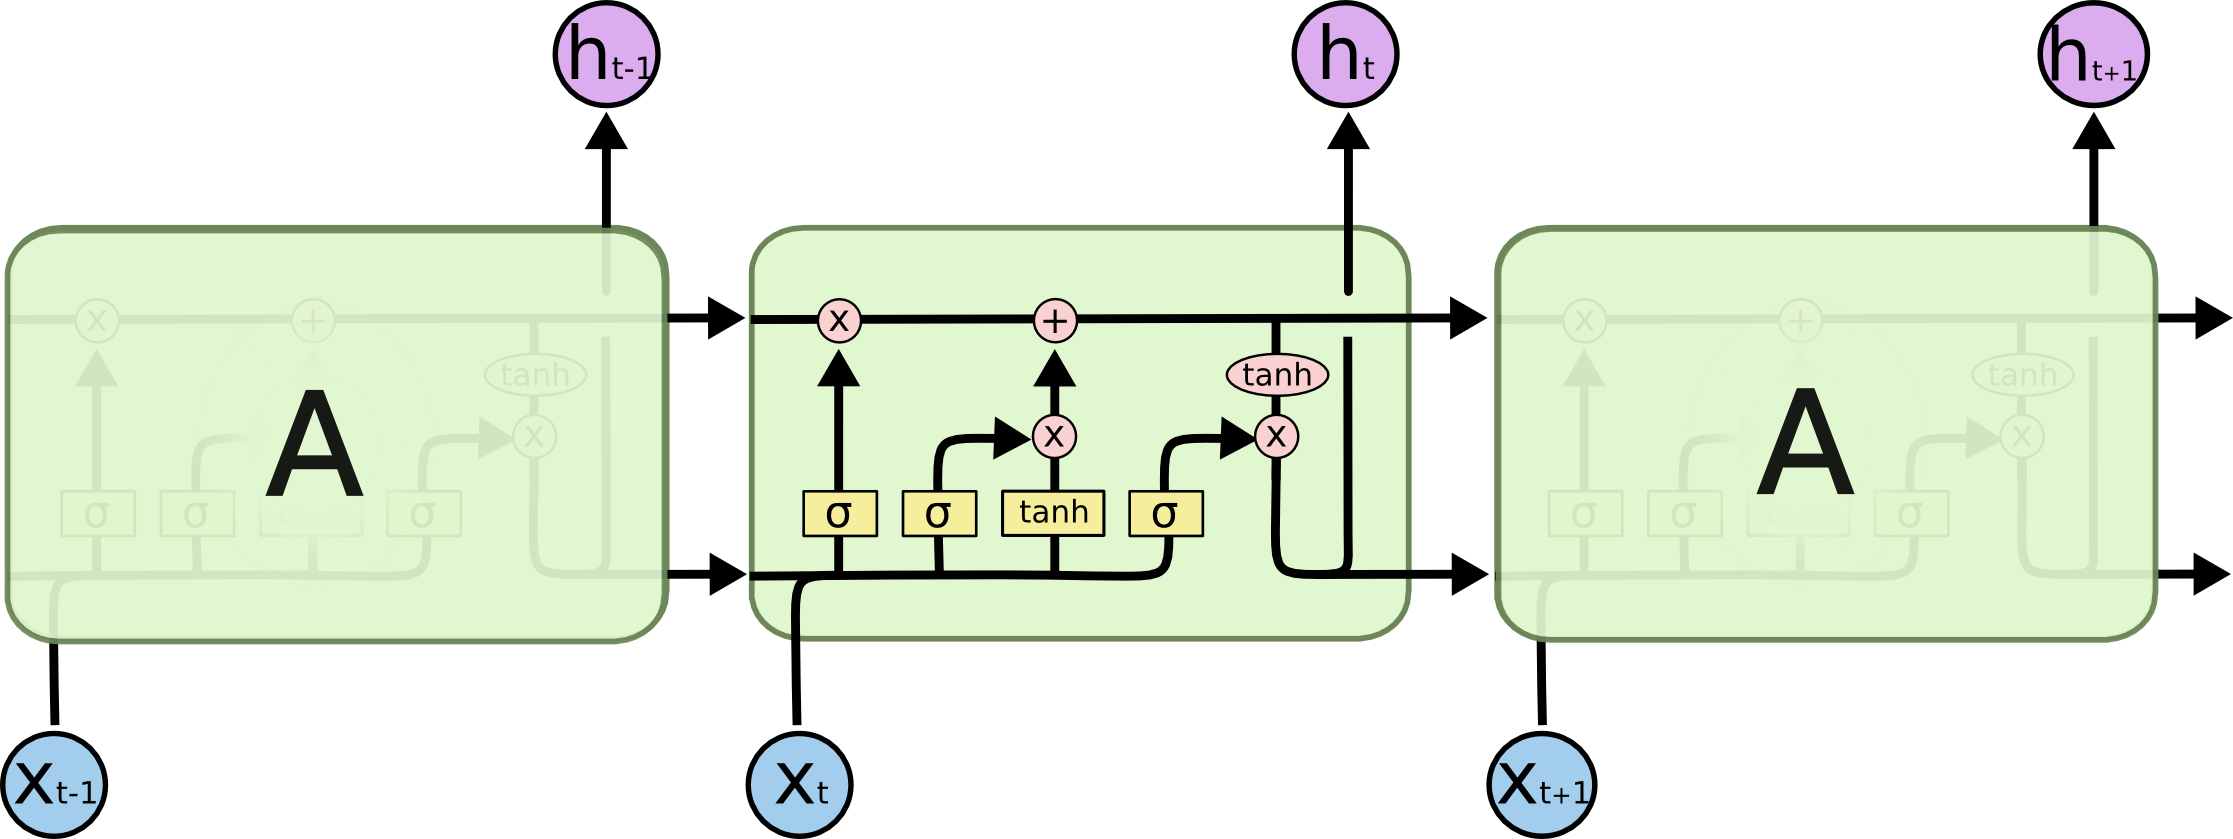
\includegraphics[width=14cm]{./Chapitre3/figures/lstm.png}
  \caption{Représentation schématique d'un réseau récurrent à mémoire court et long terme (LSTM). On observe qu'il y a deux entrées à l'unité neuronale : l'état de la cellule (cell state) en haut et la sortie classique d'un neurone en bas. Image provenant de http://colah.github.io/posts/2015-08-Understanding-LSTMs/ .}
  \label{fig:lstm}
\end{figure}


Les réseaux récurrents à mémoire court et long terme (LSTM pour long-short term memory en anglais)~\cite{Hochreiter1997} ont été crées pour répondre à la perte de la mémoire longue des RNN. Ils sont spécialisés dans la modélisation de dépendances éloignées dans une séquence, en fonctionnant avec une mémoire interne à chaque neurone, comme explicité sur la figure~\ref{fig:lstm}. La mémoire interne du neurone, appelée cell state, permet de modéliser des dépendances à des instants éloignés dans la séquence.

Lorsque la sortie de l'unité neuronale précédente $t$-$1$ arrive dans l'unité courante $t$, elle va passer par trois portes, utilisant des sigmoïdes et des tangentes hyperboliques. La première porte, la porte de l'oubli, est en charge de la suppression d'informations dans la cell-state. La deuxième porte, la porte d'entrée, va décider des nouvelles informations à ajouter dans la cell-state. La cell-state est alors mise à jour avec les informations ajoutées et retirées. La dernière porte, la porte de sortie, est en charge de la sortie effective. Elle est calculée en fonction de la cell-state mais aussi de l'état courant en utilisant une tangente hyperbolique pour forcer les valeurs entre -1 et 1 puis une dernière sigmoïde afin de ne transmettre que les informations activées.

Cette architecture existe également de façon bidirectionnelle : la séquence est lue dans l'ordre chronologique ainsi que de la fin vers le début. Pour avoir ces deux directions, on multiplie le nombre de couches du système par deux : une prenant les informations dans l'ordre et une autre prenant les informations dans l'ordre inverse. Enfin les sorties des deux couches sont concaténées pour donner la sortie finale de chaque élément. Cela permet de mettre en évidence les dépendances passées et futures.

\subsection{Encodeur Décodeur}
\begin{figure}[h]
  \centering
  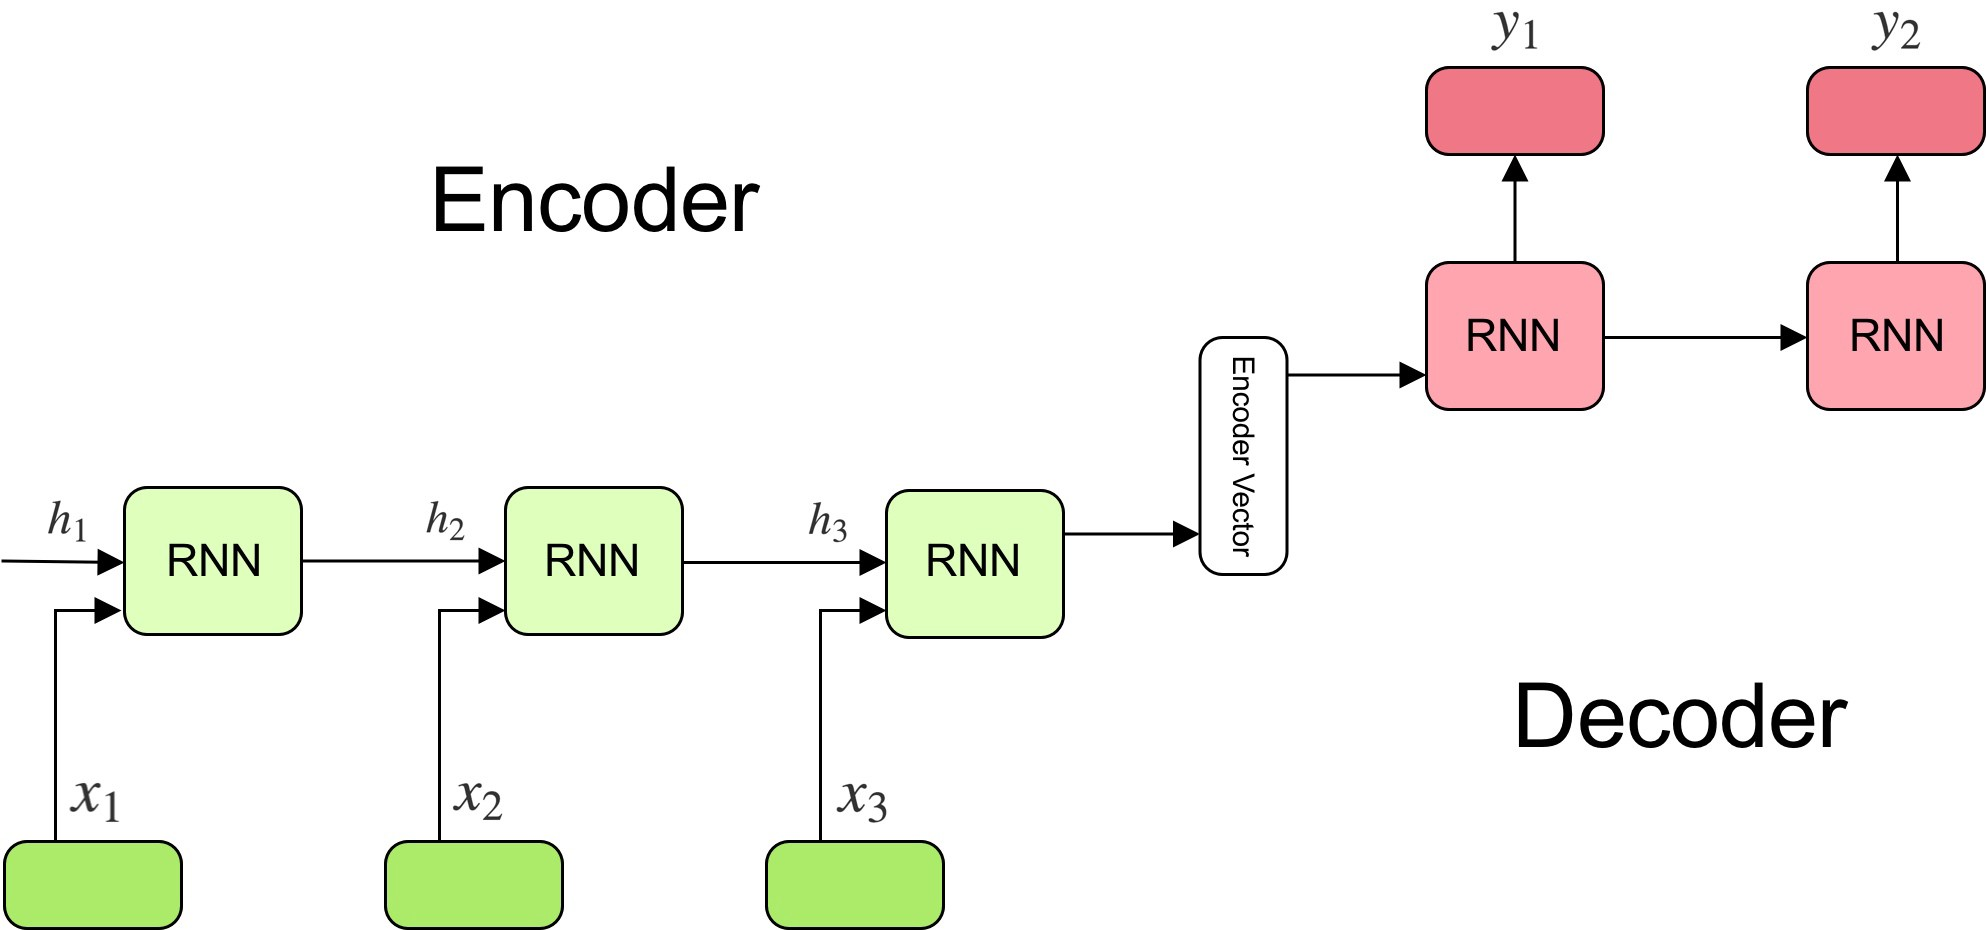
\includegraphics[width=14cm]{./Chapitre3/figures/encoder.jpeg}
  \caption{Représentation schématique d'un système encodeur décodeur. $x_i$ correspondent aux entrées, $y_i$ aux sorties. Image provenant de shorturl.at/dmsCS}
  \label{fig:encoder}
\end{figure}


Conçu dans les années 2010, l'encodeur décodeur (Encoder-Decoder en anglais)~\cite{Cho2014} se compose, comme son nom l'indique, de deux parties distinctes. Ces deux parties, l'encodeur et le décodeur sont utilisés conjointement pour prédire une ou plusieurs sorties comme illustré par la figure~\ref{fig:encoder}.

Un encodeur correspond à un réseau de neurones récurrents qui transforme une séquence d'entrée $X$ en une représentation vectorielle de taille fixe $X'$. Une fois cette première transformation effectuée, le décodeur, correspondant lui aussi à un RNN, transforme cette représentation intermédiaire $X'$ en une séquence de sortie $Y$. Cette transformation finale est calculée en fonction de la distribution de probabilité de toutes les sorties possibles $P(Y|X')$.

Cette architecture a notamment prouvé sa pertinence dans des tâches de reconnaissance de la parole~\cite{Chiu2018} ou dans des tâches de NLP~\cite{Hu2019}.

\section{SER : Speech Emotion Recognition}
Le domaine du Speech Emotion Recognition, ou reconnaissance d'émotion dans la parole en français, se concentre sur les tâches de reconnaissance des différents états émotionnels d'un ou plusieurs locuteurs. Ce domaine étant plutôt récent, il est en plein expansion grâce notamment à l'utilisation de nouveaux systèmes neuronaux empruntés à la reconnaissance automatique de parole.
Mais afin de mettre en place des expérimentations sur ces tâches de reconnaissances et de caractérisations des émotions, il est important de mettre en place des données pertinentes sur lesquelles s'appuyer, des méthodes pour représenter efficacement ces données ainsi que mettre en place des systèmes d'évaluation robustes permettant de comparer les différentes expérimentations.

\subsection{Les Corpus existants}
Aujourd'hui, les tâches de reconnaissances d'émotions sont principalement traitées en tant que tâches supervisées. Il est donc nécessaire d'utiliser des données pour réaliser des expérimentations.

\subsubsection{Corpus actés}
Comme nous l'avons vu dans le premier chapitre de cette thèse, la caractérisation en émotions d'une personne peut être assez délicate, puisqu'elle est en grande partie subjective. De plus, il est communément admis que les états émotionnels sont ponctuels et diffus dans la parole. Pour palier à ce problème, on construit des corpus dit \textit{actés}. Il s'agit de corpus où l'état émotionnel n'est pas naturel. Deux grandes possibilités existent pour construire ce genre de corpus :
\begin{itemize}
  \item soit on fait appel à des acteurs, qui vont simuler des états émotionnels dictés par le responsable de l'élaboration du corpus. Par exemple, les acteurs devront dire le mot \textit{hippopotame} de façon joyeuse, triste puis avec dégoût. Cette pratique est très utilisée pour avoir différents états émotionnels d'un même locuteur, le tout rapidement. Elle est à privilégier quand on recherche l'exhaustivité des états émotionnels chez un sujet. Ces corpus sont aujourd'hui majoritaires. Les inconvénients d'un tel protocole sont que les émotions retirées sont exacerbées dans leur manifestation, les rendant difficile à comparer à des émotions dites \textit{naturelles}. De plus, l'utilisation d'acteurs peut se révéler coûteux.
  \item soit on utilise différentes méthodes pour induire les états émotionnels que l'on souhaite étudier. Par exemple, dans le cadre de la recherche de stress, on peut présenter aux sujets des images stressantes ou leur demander de résoudre des problèmes dans un temps court. Quant à la tristesse, on peut demander aux participants de visualiser un film triste en amont. Ces émotions sont plus proches des émotions réelles, elles sont donc moins manifestes.
\end{itemize}

Les corpus actés ont pour avantage d'être créer dans des environnements contrôlés et permettent de rendre les données facilement accessibles. En effet, ces données sont produites à des fins d'analyse. Il est donc facile de recueillir le consentement des participants avant la mise en place de l'expérience, de contrôler la qualité des enregistrements et la cohérence des données en contraignant les participants sur un sujet ou à exprimer un type d'état émotionnel défini.

Les corpus les plus utilisés de nos jours sont le Berlin Emotional database, aussi appelé EMO-DB et IEMOCAP. Comme on peut le voir dans le tableau~\ref{tab:corpus}, il s'agit de deux corpus annotés selon des catégories discrètes. EMO-DB~\cite{Burkhardt2005} est composé de phrases courtes allemandes prononcées par 10 acteurs et est annoté en peur, colère, joie, tristesse, dégoût, ennui et neutre. IEMOCAP~\cite{Busso2007} est composé de conversations scriptées entre deux acteurs et est annoté en peur, colère, joie, tristesse, dégoût, frustration, surprise, excitation, neutre et \textit{autres} pour toutes les autres émotions. Joué par 10 acteurs également, cette base de données est composée de 12 heures d'audio, ce qui lui permet d'être compatible avec des approches neuronales profondes, bien qu'on préfère généralement travailler avec un plus gros volume de données.


\subsubsection{Corpus non actés}
Les corpus non actés, aussi appelés naturels ou \textit{real-life} sont obtenus directement à partir de données issues de la vraie vie. Contrairement au corpus acté, ils proviennent donc d'environnements non contrôlés où les participants n'ont pas connaissances de leur implication dans l'expérimentation à priori. Le recueil de ce type de données est facile, puisqu'il n'y a pas besoin de mettre en place un environnement spécifique. On peut directement récupérer des enregistrements provenant de débats télévisés, de reportages, de vidéos internet ou de centre d'appels par exemple.
Ces données sont donc constituées d'états émotionnels spontanés. Ces derniers sont moins marqués et identifiables que des émotions actées et ne sont pas présent sur la majorité de l'enregistrement. Le principal inconvénient de ces corpus vient de la difficulté de les diffuser. En effet, les participants n'ayant pas été prévenus en amont, il est souvent difficile de diffuser de telles données. Soit les participants doivent être retrouvés et donner leurs consentement à postériori, soit les données doivent être anonymisées pour respecter les droits des individus. De même, il est difficile d'avoir tous les états émotionnels de tous les locuteurs et de garantir une qualité d'enregistrement identique entre tous les documents.
De plus, l'étiquetage de ces données est souvent plus complexe, puisque le cadre expérimental n'a pas été expliqué aux participants.

\begin{table}[]
\begin{tabular}{|l|c|c|c|c|l|}
\hline
\textbf{Nom du Corpus}                              & \multicolumn{1}{l|}{\textbf{Langue}} & \multicolumn{1}{l|}{\textbf{Tél}} & \multicolumn{1}{l|}{\textbf{Acté}} & \multicolumn{1}{l|}{\textbf{Continue}} & \textbf{Domaine}                  \\ \hline
% \begin{tabular}[c]{@{}l@{}}DECODA
%   \\~\cite{Lailler2016}\end{tabular}                & FR                                   & o                                 & --                                      & --                                     & Transport en commun               \\ \hline
% \begin{tabular}[c]{@{}l@{}}MEDIA
%   \\~\cite{BonneauMaynard2005}\end{tabular}              & FR                                   & o                                 & --                                      & --                                     & Réservation hôtel                 \\ \hline
% \begin{tabular}[c]{@{}l@{}}PORTMEDIA
%   \\~\cite{Lefevre2012}\end{tabular}                & FR                                   & o                                 & --                                      & --                                     & Réservation ticket                \\ \hline
\begin{tabular}[c]{@{}l@{}}EMO-DB
  \\~\cite{Burkhardt2005}\end{tabular}              & Allemand                                   & x                                 & o                                       & x                                      & Mot isolés                           \\ \hline
\begin{tabular}[c]{@{}l@{}}DES
  \\~\cite{Engberg1997}\end{tabular}                & Danois                                   & x                                 & o                                       & x                                      & Mots isolés                           \\ \hline
\begin{tabular}[c]{@{}l@{}}INTERFACE
  \\~\cite{Hozjan2002}\end{tabular}                & Multi                                   & x                                 & o                                       & x                                      & Mots isolés                           \\ \hline
\begin{tabular}[c]{@{}l@{}}SUSAS
  \\~\cite{Hansen1997}\end{tabular}                & Anglais                                   & x                                 & o                                       & x                                      & Stress induit                           \\ \hline
  \begin{tabular}[c]{@{}l@{}}IEMOCAP
    \\~\cite{Busso2007}\end{tabular}                & Anglais                                   & x                                 & o                                       & x                                      & Conversations Scriptées                           \\ \hline
\begin{tabular}[c]{@{}l@{}}CallSurf
  \\~\cite{Garnier2008}\end{tabular}                & Français                                   & o                                 & x                                       & x                                      & Energie                           \\ \hline
\begin{tabular}[c]{@{}l@{}}Natural
  \\~\cite{Morrison2007}\end{tabular}               & Chinois                              & o                                 & x                                       & x                                      & Energie                           \\ \hline
\begin{tabular}[c]{@{}l@{}}Conversation d'urgence
  \\~\cite{Devillers2010}\end{tabular}              & Français                                   & o                                 & x                                       & x                                      & Centre d’urgence                  \\ \hline
\begin{tabular}[c]{@{}l@{}}RECOLA
  \\~\cite{Ringeval2013}\end{tabular}               & Français                                   & x                                 & x                                       & o                                      & Vidéo conférence                  \\ \hline
\begin{tabular}[c]{@{}l@{}}SEMAINE
  \\~\cite{McKeown2012}\end{tabular}                & Anglais                                 & x                                 & o                                       & o                                      & Conversation SAL                  \\ \hline
\begin{tabular}[c]{@{}l@{}}\textbf{SEWA}
  \\~\cite{SEWA}\end{tabular}               & \textbf{Multi}                       & \textbf{x}                        & \textbf{x}                              & \textbf{o}                             & \textbf{Commentaire de publicité} \\ \hline
\end{tabular}
\caption{Principaux corpus utilisés dans la reconnaissance d'émotions dans la parole. Chaque corpus est caractérisé par la langue utilisée, si les enregistrements sont issus du domaine téléphonique ou non, s'il s'agit d'un corpus acté ou spontanée et si les émotions sont annotées en continue ou non.}
\label{tab:corpus}
\end{table}


Les principaux corpus actés et non actés, utilisés dans la reconnaissance automatique d'émotion, sont listés dans le tableau~\ref{tab:corpus}. Nous avons citer en particulier le corpus RECOLA et le corpus SEWA. Ces deux corpus sont particulièrement adaptés à notre tâche, puisqu'ils sont annotés selon des émotions continues.
RECOLA~\cite{Ringeval2013} est constitué de conversations dyadiques effectuées en visioconférence pendant laquelle les deux participants doivent compléter une tâche qui leur demande de coopérer. La base de données est notamment constituée des 5 premières minutes de l'enregistrement audio des 23 binômes ainsi formés, totalisant 3 heures et 50 minutes d'audio. 6 annotateurs ont mesurés les états de valence et d'activation des participants.
SEWA~\cite{SEWA} est constitué de conversations entre deux locuteurs concernant des publicités visualisées en amont. Le corpus est notamment constitué des enregistrements audio de ces conversations réalisées en 6 langues différentes et réunissant 398 participants pour un total de 44 heures. Ces deux corpus sont disponibles pour les membres d'institution de recherche, en faisant des corpus de plus en plus utilisés.

Dans le cadre de cette thèse, nous avons décidé de comparer nos résultats à ceux obtenus avec le corpus SEWA, comme il se rapproche sur plusieurs points de notre problématique.


\subsection{Features}
Afin de valoriser les données que nous avons dans les différents corpus, il est important de mettre en place une transformation pertinente des données brutes en features, aussi appelés caractéristiques ou descripteurs en français.
Ces features proviennent des domaines de la phonétique notamment et de la reconnaissance de la parole ou de la musique. Leur but est de mesurer les caractéristiques phonatoires et articulatoires des locuteurs~\cite{Scherer1986} afin d'extraire les informations linguistiques et para-linguistiques du discours.

\subsubsection{Spectrogramme}
\begin{figure}[h]
  \centering
  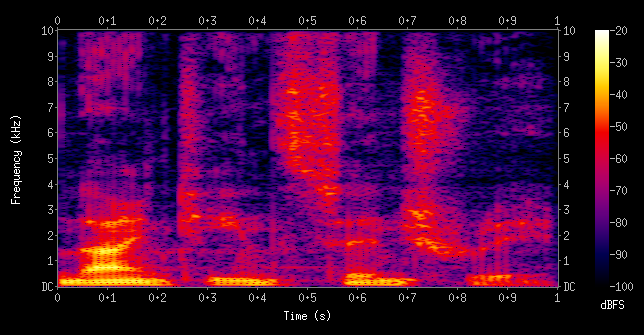
\includegraphics[width=12cm]{./Chapitre3/figures/spectrogramme.png}
  \caption{Représentation du signal en tant que spectogramme. La fréquence est modélisée en ordonnée et le temps en abscisse. L'énergie est visible grâce aux couleurs présentes: plus la couleur est chaude (rouge, orange, jaune) et plus l'énergie dégagée est importante. Image provenant de Wikipedia.}
  \label{fig:spectrogramme}
\end{figure}


Un spectrogramme est une représentation du signal audio mettant en avant l'énergie en fonction de la fréquence et du temps. Comme on peut le voir sur la figure~\ref{fig:spectrogramme}, il s'agit d'une représentation tridimensionnelle du signal audio. Cette transformation est possible en utilisant la transformation de Fourier qui permet de passer de l'espace temporel à l'espace fréquentiel. Une fois cette transformation effectuée, on peut calculer le spectre du signal par fenêtre d'observation. Ainsi, les zones les plus chaudes (jaune/orange) de la figure correspondent aux énergies les plus fortes, que l'on appelle des formants.

Cette représentation est souvent utilisé lorsque l'on considère le signal audio comme une image. On est ainsi capable d'utiliser des systèmes de reconnaissance d'images afin de traiter des problématiques touchant au domaine de la parole~\cite{Stolar2017}.


\subsubsection{Coefficients Cepstraux de Fréquence de Mel}
Les MFCCs, Mel-Frequency Cepstral Coefficients en anglais, sont des descripteurs spectraux qui sont extraits sur des petites fenêtres du signal audio. Ils sont issus d'un ensemble de traitement qui est appliqué sur le signal audio traditionnellement sur des fenêtres temporelles de 30 ms tous les 10ms. Cette extraction correspond à l'énergie du signal ainsi qu'au 12 premiers coefficients cepstraux. Afin de modéliser l'évolution temporelle du signal, on utilise les dérivées premières et secondes de ces coefficients. Contrairement aux autres représentations spectrales telles que le Linear Predictive Coding (LPC)~\cite{Rabiner1993} ou les Perceptual Linear Prediction (PLP)~\cite{Hermansky1990}, ces coefficients sont adaptés à l'audition humaine puisqu'ils suivent l'échelle de perception de Mel. En effet, notre perception des sons n'est pas linéaire : nous percevons plus de différence entre des sons de 1000 et 2000 kHertz qu'entre des sons de 7000 et 8000 kHertz.

Au total, nous avons donc une représentation en vecteurs de taille 39 pour chaque fenêtre de 10ms de signal, nous permettant de réduire considérablement le signal d'entrée, tout en gardant les informations essentielles contenues dans l'audio.

\subsubsection{Ensemble de descripteurs}
Dans le domaine du Speech Emotion Recognition, il n’y a pas de consensus sur le meilleur ensemble de descripteurs à utiliser pour effectuer des tâches de reconnaissance d'émotions. C'est pour cela qu'il existe un grand nombre de set de descripteurs regroupant les différents indices acoustiques mis en relation avec les émotions. Ces indices sont soit extraits au niveau de fenêtres de courtes durées (30ms le plus souvent), soit sur des fenêtres plus longues (plus d'une seconde) pour capturer les phénomènes para-linguistiques.

Traditionnellement, on prend un très grand nombre de descripteurs, comme par exemple le set de base extrait avec OpenSMILE~\cite{OPENSMILE}, qui compte 988 descripteurs acoustiques, puis on les filtre pour conserver les plus pertinents. Néanmoins l'ordre de grandeur des corpus annotés en émotion peut vite poser problème si la dimension des descripteurs est trop importante.

Pour palier à ces problèmes, de plus petits ensembles de descripteurs, réalisés par des experts du domaine ont été proposés dont \textit{The Geneva Minimalistic Acoustic Parameter Set} (GeMAPS) et sa version étendue (eGeMAPS)~\cite{Eyben2016}. Il est composé de 25 descripteurs de bas niveau (Low Level Descriptors en anglais)  représentant des propriétés de fréquence, d’énergie, d’amplitude et des propriétés spectrales. Comme la version courte de l’ensemble minimaliste ne contient aucun paramètre spectral et très peu de paramètres dynamiques, cinq LLD définis dans l’ensemble d’extension comportant des paramètres spectraux sont ajoutées. Le tableau~\ref{tab:egemaps} résume toutes les caractéristiques retenues dans cet ensemble.

\begin{table}[h]
   \centering
   \begin{tabular}{| l |}
   \hline
       Paramètres fréquentiels \\
   \hline
       Hauteur de la voix (Pitch)  \\
       Tremblement de la voix (Jitter) \\
       Frequence des Formants 1,2,3 \\
       Bande passante (Bandwidth) des Formants 1,2,3 \\
   \hline
       Paramètres d'énergie et d'amplitude \\
   \hline
       Scintillement (Shimmer) \\
       Volume (Loudness) \\
       Ratio Harmonique-Bruit (Harmonics-to-Noise Ratio) \\
   \hline
       Paramètres spectraux \\
   \hline
       Ratio Alpha \\
       Index de Hammarberg \\
       2 pentes spectrales : 0-500Hz et 500-1500Hz \\
       Energie relative des Formants 1,2,3 \\
       Différence harmonique H1-H2 et H1-A3 \\
       MFCC 1 à 4 \\
       Flux spectral \\
   \hline
       Paramètres temporels  \\
   \hline
       Taux des pics de volume (Rate of loudness peaks) \\
       Moyenne et variance des zones parlées \\
       Moyenne et variance des zones non parlées \\
       Nombre de zones continues parlées par secondes \\
   \hline

   \end{tabular}
   \caption{Résumé des descripteurs de bas niveau (LLDs) utilisés dans l'ensemble eGeMAPS.}
   \label{tab:egemaps}
\end{table}


% \subsubsection{Bag-of-Audio-Words}
% Comme nous l'avons déjà indiqué, la sélection de la représentation de l'audio est un choix qui va directement influencer la qualité de la reconnaissance des émotions. C'est pour cela qu'il existe de nombreuses représentations, dont les sacs de mots-audio, ou BoAW. Inspiré des sacs de mots utilisés en NLP, il s'agit d'utiliser des LLDs sélectionnés pour former un lexique de toutes les valeurs possibles, puis de les coder par un vecteur. Ce vecteur est alors utilisé en tant qu'entrée du système.
% Cette solution présente comme avantage de renforcer la robustesse du système, vu que les LLDs en entrées sont en quelque sorte normalisées par ce processus. Ces features sont utilisées dans de nombreuses tâches reliées à la parole : la classification d'évènements sonores ou la détection de musique par exemple. Ils ont également été utilisés en reconnaissance d'émotion continue.
%In this approach, feature vectors of acoustic LLDs are quantised according to a learnt codebook of audio words. Then, a histogram of the occurring ‘words’ is built.


\subsection{Évaluation des performances}
De nombreuses mesures ont été utilisées au fur et à mesure de l'avancé du domaine pour évaluer les performances des systèmes de reconnaissance d'émotions dans la parole. L'un des premier, le f-score a vite fait place à l'accuracy (précision) avant que des campagnes d'évaluation mettent en place le Coefficient de Corrélation de Concordance (CCC) comme la mesure la plus usité dans l'évaluation de systèmes de reconnaissance de l'émotion continue.

\subsubsection{Matrice de confusion et scores associés}
La matrice de confusion est une matrice permettant de mesure la performance d'un système de classification. Elle est donc mise en place en tant qu'évaluation lorsque les émotions sont de nature discrètes. Grâce à elle, on peut retrouver les différentes erreurs du système et les quantifier. Un exemple de matrice de confusion est donné par le tableau~\ref{tab:matriceConf}. Les lignes correspondent aux références, et les colonnes aux prédictions d'un système.

\begin{table}[h]
  \centering
\begin{tabular}{|l|l|c|c|c|c||c|c|}
\cline{3-6}
\multicolumn{1}{c}{}       &         &\multicolumn{4}{c||}{\textbf{Prédiction}} \\ \cline{4-8}
\multicolumn{1}{c}{}       &             & joie        & neutre      & colère &total      &précision &rappel\\ \hline
\multirow{3}{*}{\rotatebox[origin=c]{90}{\textbf{Réf}}} &joie   & \textbf{90} & 11          & 2 &103                &0.900 &0.874\\ \cline{2-7}
                     & neutre & 4           & \textbf{80} & 10       &94        &0.889 &0.851 \\ \cline{2-8}
                     & colère & 6           & 9           & \textbf{20} &35      &0.625 &0.571 \\ \cline{2-8} \cline{2-8}
                     %& total  & 100         & 90          & 32           & & \\ \hline
\end{tabular}
\caption{Matrice de Confusion entre trois classes émotionnelles : la joie, le neutre et la colère. Les colonnes correspondent aux prédictions du système et les lignes correspondent aux références. On voit que sur 100 prédictions de la classe joie, seules 90 sont pertinentes et le système a mal prédit 13 segments qui ne devraient pas être dans la classe joie.}
\label{tab:matriceConf}
\end{table}

\begin{figure}[h]
  \centering
  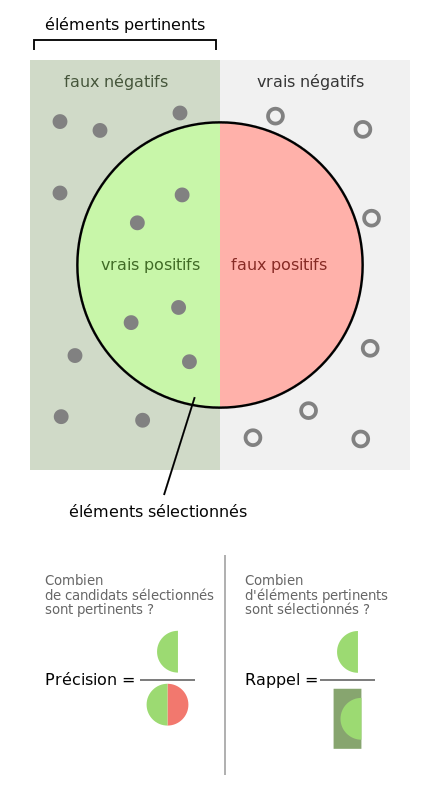
\includegraphics[width=7cm]{./Chapitre3/figures/precisionRappel.png}
  \caption{Représentation schématique de la précision et du rappel. Image provenant de Wikipedia}
  \label{fig:precisionRappel}
\end{figure}


Cette présentation permet notamment de visualiser si une classe est plus prédite que d'autres. Il est facile de relever si le système est performant en se basant sur la diagonale, qui regroupe les vrais positifs, tandis que les autres cases correspondent à des erreurs du système.

Cette matrice de confusion permet également de calculer le rappel et la précision de chaque classe, illustré dans la figure~\ref{fig:precisionRappel}. La précision correspond au nombre de documents pertinents retrouvés parmi tous les documents. Le rappel correspond au nombre de documents pertinents retrouvés parmi tous les documents pertinents.

Bien que pratique, la matrice de confusion ne permet pas de donner un score unique pour le système. C'est pour cela que la communauté s'est tournée vers l'accuracy pondérée.

\vspace{1cm}
% \\
\textit{Précision pondérée et non-pondérée}

Afin d'avoir un score global de la classification des émotions, on utilise principalement la précision pondérée (WA pour weighted accuracy) comme dans les travaux de Lee et Tashev~\cite{Lee2015} ou de Han et al.~\cite{Han2014}.
La WA compare le nombre total de documents correctement prédits au nombre total de documents selon l'équation~\ref{eq:WA}. Si on se réfère à la matrice de confusion, il suffit d'additionner toute la diagonale et de diviser par le nombre total de documents.

\begin{equation}
  WA = \frac{nb  prediction_{ok}}{nb  prediction_{totale}}
  \label{eq:WA}
\end{equation}

Cette mesure permet de calculer la performance d'un système de reconnaissance, mais elle ne prend pas en compte la différence de performance entre les classes. Par exemple, la classe colère dans notre exemple est peu performante. Pourtant si on calcule la WA ($\frac{90+80+20}{100+100+32}$) on retrouve $0,82$ soit $82\%$ de bonne prédiction. Hors les prédictions de la classe colère ont une précision de $63\%$.

Il est donc utile de compléter cette mesure de performance par la précision non-pondérée (UA pour unweighted accuracy), qui va faire la somme des précisions de chaque classes. Ici nous ferons la somme des précisions des trois classes.

\vspace{1cm}
\textit{F-mesure}

La F-mesure, ou F-score en anglais, combine à la fois la précision et le rappel selon l'équation~\ref{eq:Fmesure}. Elle est comprise entre 0 et 1. Plus elle est grande, plus le système évalué est performant.

\begin{equation}
  F = 2 \left( \frac{precision.rappel}{precision+rappel} \right)
  \label{eq:Fmesure}
\end{equation}

Néanmoins toutes les reconnaissances d'émotion ne se font pas sur des émotions discrètes, il existe donc d'autres indicateurs utilisés pour mesurer la performance des systèmes.

\subsubsection{Racine de l'erreur quadratique moyenne}
La racine de l'erreur quadratique moyenne, RMSE pour Root Mean Square Error, est une métrique qui est utilisé dans l'évaluation des systèmes de reconnaissance d'émotions continues~\cite{AVEC2017}. Elle permet de calculer un score d'accord entre deux séries temporelles, ici les annotations de références et les prédictions du système. Cette métrique se calcule selon l'équation~\ref{eq:RMSE_score} avec $x_i$ correspondant aux prédictions, $y_i$ aux références et $n$ la longueur des séries.

\begin{equation}
    RMSE = \sqrt{\frac{1}{n}\Sigma_{i=1}^{n}{\Big(y_i - x_i\Big)^2}}
\label{eq:RMSE_score}
\end{equation}

Elle est comprise entre 0 et 1. Comme il s'agit d'un taux d'erreur, les systèmes à haute performance se rapproche de 0, ce qui indique un ajustement parfait entre les références et les prédictions. Cette métrique n'est pas exempte d'inconvénient. En effet, elle est très sensible aux valeurs extrêmes.

\subsubsection{Coefficient de Corrélation de Concordance}
Le coefficient de corrélation de concordance~\cite{CCC}, CCC pour Concordance Correlation Coefficient, a été établi comme un standard d'évaluation lors notamment des trois précédents Audio/Visual Emotion Challenge and Workshop (AVEC)~\cite{AVEC2017,AVEC2018,AVEC2019}. Cette métrique évalue l'accord entre deux séries temporelles selon l'équation~\ref{eq:CCC_score}, où $x$ et $y$ sont les deux variables temporelles, dans notre cas la prédiction et la référence. $\mu_x$, $\mu_y$ correspondent à leurs moyennes et $\sigma_x$, $\sigma_y$ à leur écart-type.

 \begin{equation}
    CCC = \frac{2\rho\sigma_x\sigma_y}{\sigma_x^2 + \sigma_y^2 + (\mu_x - \mu_y)^2}
 \label{eq:CCC_score}
 \end{equation}

Plus le CCC s'approche de 1 et plus le système est considéré comme performant. A l'inverse, plus le score s'approche de 0 et moins il y a de corrélation entre les prédictions et les références, dénotant un système peu performant.

Cette métrique sera utilisé dans les travaux de cette thèse pour évaluer la performance des systèmes.

\subsection{Les scores de systèmes à l'état de l'art tirés d'AVEC}

\begin{table}[]
    \centering
    \begin{tabular}{| l | l | l | c | c | c |}
        \hline
        \textbf{Models} &\textbf{Modalité} &\textbf{Features} &\multicolumn{3}{c|}{\textbf{SEWA}} \\ \cline{3-6}
        & & &activation &valence &liking \\
        \hline
        \multicolumn{6}{|l|}{AVEC 2017~\cite{AVEC2017} : Sur les conversations allemandes} \\
        \hline
        SVR      &audio &BoAW~\cite{Schmitt2016} &.344  &.351 &.081 \\
        SVR      &audio &BoTW                    &.373  &.390 &.314 \\
       \hline
       \multicolumn{6}{|l|}{Huang et al.~\cite{Huang2017} : Sur les conversations allemandes} \\
       \hline
       LSTM     &audio &eGeMAPS-88  &.506  &.455 &.193 \\
       LSTM     &audio &IS10        &.465  &.440 &.227 \\
       LSTM     &audio &Bottle-neck~\cite{Fer2015} &.533  &.466 &     \\
       LSTM     &audio &Mfcc        &.341  &.421 &     \\
       LSTM     &texte &BoTW        &.451  &.518 &.473 \\
        \hline
        \multicolumn{6}{|l|}{AVEC 2018~\cite{AVEC2018} : Sur les conversations allemandes} \\
        \hline
        biLSTM-2 &audio &eGeMAPS-88  &.124  &.112 &.001 \\
        biLSTM-2 &audio &Mfcc        &.253  &.217 &.136 \\
         \hline
       \multicolumn{6}{|l|}{Huang et al.~\cite{Huang2018} : Sur les conversations allemandes} \\
       \hline
       LSTM     &audio &eGeMAPS-88   &.497  &.438 &.281 \\
       LSTM     &audio &eGeMAPS-89   &.520  &.461 &\textbf{.335} \\
       LSTM     &audio &eGeMAPS-176  &.514  &.493 &.217 \\
       LSTM       &texte &Word2Vec-300   &\textbf{.597}  &\textbf{.600} &.454 \\
       LSTM-2     &texte &BoW            &  & &.407 \\
       LSTM-2     &texte &Word2Vec       &  & &\textbf{.480} \\
       LSTM-2     &texte &GloVe          &  & &.413 \\
        \hline
        \multicolumn{6}{|l|}{AVEC 2019~\cite{AVEC2019} : Sur les conversations allemandes et hongroises} \\
        \hline
        biLSTM-2 &audio &eGeMAPS-88  &.371 &.286 &.159 \\
        biLSTM-2 &audio &Mfcc        &.326 &.187 &.144 \\
         \hline
       \multicolumn{6}{|l|}{Schmitt et al.~\cite{Schmitt2019} : Sur les conversations allemandes} \\
       \hline
       \rowcolor{Red}
       CNN      &audio &eGeMAPS-47    &\textbf{.571}  &.517 & \\
       \rowcolor{Red}
       biLSTM-4 &audio &eGeMAPS-47    &.568  &\textbf{.561} & \\
       \hline
    \end{tabular}
    \caption{Compilation des scores de CCC sur l'ensemble de développement de SEWA sur les 3 dimensions : activation, valence et \textit{liking}. L'acronyme BoAW signifie \textit{Bag-of-audio-words}, BoTW signifie \textit{Bag-of-text-words}, SVR signifie Support Vector Regression~\cite{Smola2004}, proche des SVM mais applicable à des problèmes de régression et donc à une annotation continue. Les différents nombres associés aux features de type eGeMAPS dénotent de différentes configurations utilisées autour de ces sets : soit avec une sélection reduite des LLDs (47), soit avec l'ajout d'information sur le locuteur courant (89 et 176).}
    \label{tab:avec}
\end{table}

Si nous nous replaçons dans le contexte de la thèse, nous cherchons à construire et donc à évaluer un système de reconnaissance des émotions continues depuis la parole. Afin de pouvoir nous comparer à l'état de l'art, nous avons décidé de comparer nos résultats à ceux obtenus sur le corpus SEWA, dont nous avons parlé plus tôt.
Ce corpus considère trois axes d'émotions continues : la valence, l'activation et le \textit{liking}. Il est utilisé notamment dans les campagnes AVEC depuis 2017~\cite{AVEC2017,AVEC2018,AVEC2019}.

Ces campagnes sont divisées en différents objectifs qui gravitent autour des émotions: de la détection de dépression, de bipolarité, d'état d'esprit ou d'émotions issues de différentes cultures par exemple. Comme ces campagnes s'appuient sur des corpus multimodaux, les émotions peuvent être détectées à partir de différentes modalités, notamment depuis la parole et les expressions faciales.

Nous présentons dans le tableau~\ref{tab:avec}, différents résultats obtenus qui utilisent la partie Allemande et Hongroise du corpus, soit celle auquel nous avons accès. Comme nous pouvons le voir, de nombreuses caractéristiques et type d'algorithme ont été utilisés pour la reconnaissance des émotions depuis la parole pour le corpus SEWA. Nous pouvons voir que les systèmes les plus performants ont des scores de 0.571 pour l'activation, 0.561 pour la valence et 0.335 pour le liking.

Dans le cadre de cette thèse, nous cherchons à mettre en place des solutions neuronales profondes. Nous avons donc fait le choix de nous comparer aux résultats obtenus par Schmitt et al.~\cite{Schmitt2019}.

\section{Sentiment Analysis et Opinion Mining}
Utiliser le texte pour déterminer l'état émotionnel est une voie de plus en plus empruntée grâce, notamment, à la performance des systèmes de reconnaissance de la parole actuels.
Des domaines tels que l'Analyse de Sentiments et la Détection d'Opinion, utilise des données textuelles de type livres, témoignages ou plus récemment des tweets et  des contenus en ligne afin d'extraire des informations. On peut également considérer la transcription automatique comme un élément associé à la parole, et donc y retrouver des marqueurs de l'émotion.

Dans ces domaines, on cherche alors l'émotion dans l'aspect sémantique de la phrase, dans les diffluences ou les répétitions.

Le terme \textit{Détection d'Opinion} (traduction de Opinion Mining) a été popularisé par les travaux de Kushal Dave~\cite{Dave2003}, définissant le domaine comme traitant un ensemble de données pour en retirer ses qualités et ses caractéristiques afin de statuer sur l'avis du sujet~\cite{Pang2008}. Le domaine \textit{Analyse de Sentiments} (traduction de Affect Analysis) a pris de l'ampleur depuis les travaux de Sanjiv Das, Mike Chen et Richard Tong au début du XXIe siècle~\cite{Das2007,Tong2001}. Il diffère de l'Opinion Mining : la majorité de ces travaux se concentrent sur la classification des avis ou de phrases en polarité (positif ou négatif). Mais ces domaines de recherche restent très fortement liés et constituent la plus grande partie de recherche d'indices émotionnelles à base de données textuelles.

Des outils tel que des dictionnaires de polarité, FAN~\cite{Monnier2014} par exemple, permettent de colorer émotionnellement des mots ou des phrases, ou encore des analyseurs de syntaxe tel que Macaon~\cite{Nasr2011} permettent d'étudier la structure d'un énoncé pour faire ressortir sa forme morphosyntaxique. Ces outils sont utilisés dans la reconnaissance d'émotions que ce soit à l'échelle d'un segment de parole, d'une phrase ou d'un document.

\subsection{Corpus existant}
De nombreux corpus de texte existent, mais peu sont annotés en émotion. Si nous nous référons aux campagnes AVEC, la transcription automatique de la parole est utilisée en tant que donnée textuelle. Cette transcription est ensuite alignée aux annotations, permettant d'obtenir ainsi des données annotées.

Il est également possible de constituer son propre corpus en confrontant un texte à des lexiques d'émotions comme par exemple le lexique NRC~\cite{Mohammad2013} disponible dans 105 langues, SentiWordNet~\cite{Sebastiani2006} ou encore le lexique FAN~\cite{Monnier2014}.
Le lexique NRC contient 14 182 mots et sont associés à 10 catégories différentes (anticipation, colère, tristesse, joie, peur, confiance, dégoût, surprise, positive, négative). Chaque mot peut être associé à plusieurs catégories ou à aucune.
Le dictionnaire French Affective Norms (FAN) propose quant à lui, un score de valence (entre 0 et 10) pour plus de 1000 mots, annotés par plus de 400 participants.

Il est également possible de se tourner vers des corpus déjà construits, comme ceux utilisés lors des campagnes SemEval. Par exemple des titres d'article provenant de journaux~\cite{Strapparava2010} ou encore un corpus constitué de livres pour enfants~\cite{Etienne2020}. Les données de SemEval sont annotés en catégories discrètes (colère, dégoût, peur, joie, tristesse, surprise et valence) par une échelle allant de 0 à 100 pour chaque émotion. 0 signifiant l'absence de l'émotion dans le titre et 100 la charge émotionnelle maximale. La valence varie entre -100 (négative) et 100 (positive) avec 0 (neutre) au milieu. Le corpus de livres pour enfants est annoté en 10 catégories discrètes (colère, dégoût, joie, peur, surprise, tristesse,culpabilité, embarras, fierté et jalousie). Cette annotation est enrichie en plusieurs concepts, notamment le mode d'expression de l'émotion : désignée, comportementale, montrée, étayée.

De nombreux autres corpus existent afin de traiter un maximum de tâches en lien avec les émotions. Mais ces corpus sont difficilement utilisables en l'état, il est important de les transformer afin de les rendre compréhensibles par les systèmes d'apprentissage.

\subsection{Features}
Dans les domaines du Sentiment Analysis et de l'Opinion Mining, nous travaillons avec des ensembles de mots. Pour les utiliser avec des algorithmes d'apprentissage, il faut transformer ces mots en séries de vecteurs de nombres.

\subsubsection{Représentation en one-hot}
La représentation en one-hot, comme illustré sur la figure~\ref{fig:onehot}, correspond à associer à chaque terme un vecteur. On rassemble tous les mots différents utilisés dans ce que l'on nomme un vocabulaire. Puis pour chaque entrée de ce vocabulaire, on associe un vecteur qui identifie l'entrée (appelé token). Cette méthode présente l'avantage d'être exhaustive, cependant la représentation est très volumineuse : le vecteur sera de la taille du vocabulaire.

\begin{figure}[h]
  \centering
  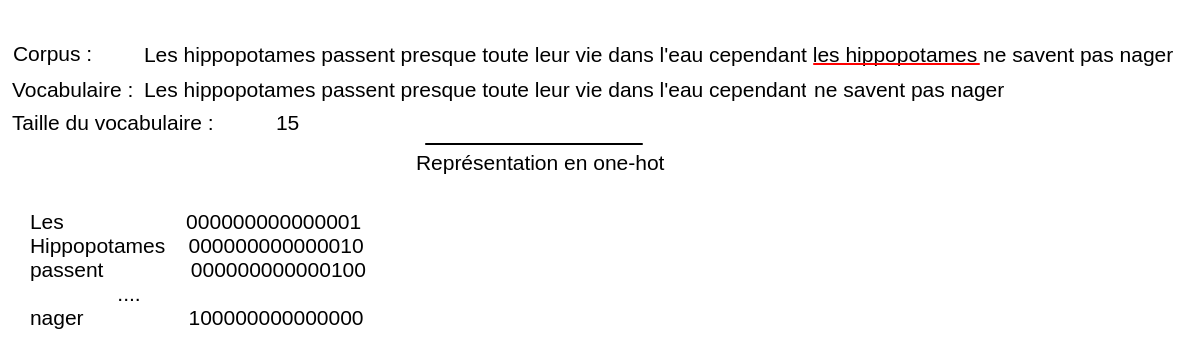
\includegraphics[width=15cm]{./Chapitre3/figures/onehot.png}
  \caption{Transformation d'un corpus en représentation one-hot.}
  \label{fig:onehot}
\end{figure}


De plus cette représentation ne porte aucune information sur la sémantique ou sur le nombre d'apparition de chaque terme.

\subsubsection{Représentation statistique}
Parmi les représentations statistiques des données, les plus courantes et les plus mises en place sont les méthodes TF (Term Frequency) et TF-IDF (Term Frequency-Inverse Document Frequency) qui prennent en compte la répartition des termes dans les documents. Pour TF, on prend le nombre d'apparition d'un terme divisé par le nombre de termes dans le document. Pour TF-IDF, on divise par l'inverse de la fréquence dans tous les documents. Ainsi, les termes qui sont trop fréquents ou présents dans tous les documents sont moins mis en avant par la représentation.

Ces méthodes statistiques ont fait leur preuve, même si on leur préfère maintenant des méthodes qui intègrent des aspects sémantiques notamment.

\subsubsection{Plongement de mots}
\begin{figure}[h]
  \centering
  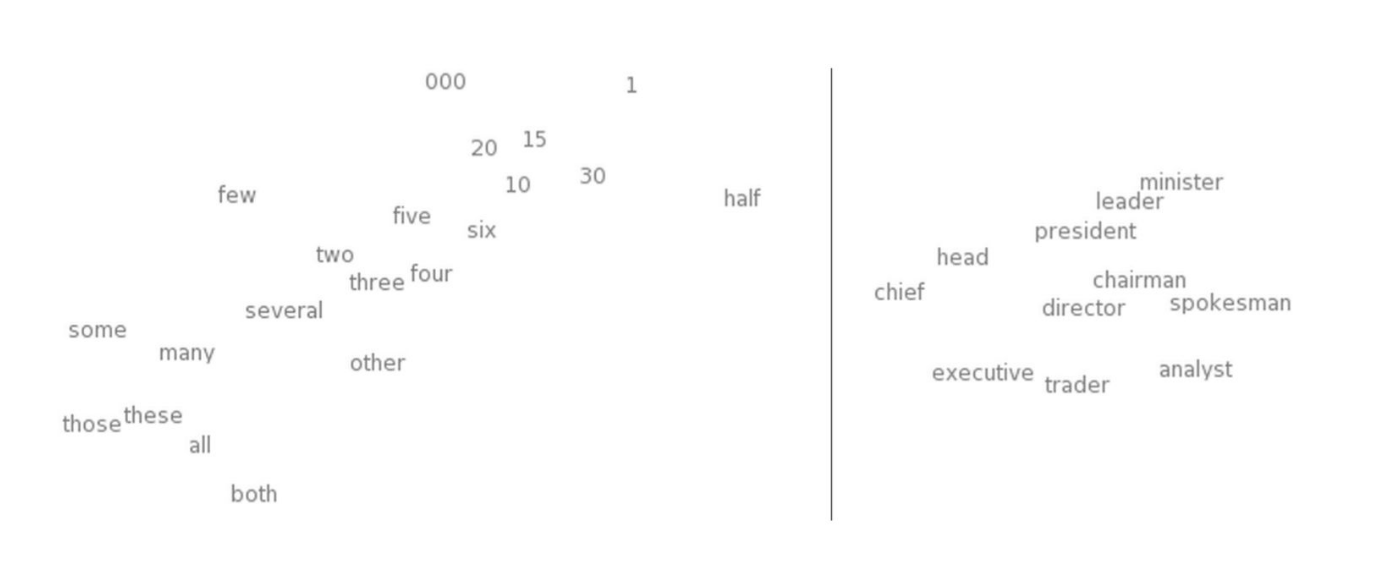
\includegraphics[width=14cm]{./Chapitre3/figures/word2vec.png}
  \caption{Représentation de plongements de mots en deux dimensions. Les mots de gauche correspondent au regroupement des termes associés au numérique. Les mots de droite correspondent aux termes associés à l'emploi. Issue des travaux de Turian et al.~\cite{Turian2010}.}
  \label{fig:word2vec}
\end{figure}


Les plongements de mots (word embeddings en anglais) ont été présentés par Bengio et al.~\cite{Bengio2003}. Ils décrivent une nouvelle représentation des mots basée sur une approche neuronale. On projète les mots dans un espace de faible dimension, tout en isolant ensemble les mots qui ont des similarités sémantiques et syntaxiques~\cite{Ghannay2017}. Chaque vecteur est ensuite inscrit ainsi dans un dictionnaire, et on peut alors remplacer chaque mot par le vecteur le représentant.

Leur utilisation et leur pertinence a été démontré dans de nombreuses tâches, notamment des tâches de TALN: l’étiquetage morphosyntaxique, la reconnaissance d’entités nommées, la détection de mention~\cite{Turian2010,Bansal2014} et de compréhension de la parole~\cite{Mesnil2013,Yao2014,Liu2016}.

Parmi les méthodes les plus utilisées on retrouve Word2vec qui peut s'apprendre avec deux algorithmes (CBOW et Skip-gram)~\cite{word2vec} ou encore GloVe~\cite{Pennington2014}.

Il est utile de noter que ce genre de représentation peuvent être visualisé dans un espace plus restreint, typiquement en deux dimensions. Ainsi les expérimentateurs peuvent observer les rapprochements sémantiques ou syntaxiques détectés par le système, comme l'illustre la figure~\ref{fig:word2vec}


\subsection{Les scores de systemes à l'état de l'art tirés d'AVEC}
\begin{table}[]
    \centering
    \begin{tabular}{| l | l | c | c | c |}
        \hline
        \textbf{Models} &\textbf{Features} &\multicolumn{3}{c|}{\textbf{SEWA}} \\ \cline{3-5}
        & &activation &valence &liking \\
        \hline
        \multicolumn{5}{|l|}{AVEC 2017~\cite{AVEC2017} : Sur les conversations allemandes} \\
        \hline
        SVR      &BoTW       &.373  &.390 &.314 \\
       \hline
       \multicolumn{5}{|l|}{Huang et al.~\cite{Huang2017} : Sur les conversations allemandes} \\
       \hline
       LSTM     &BoTW        &.451  &.518 &.473 \\
        \hline
       \multicolumn{5}{|l|}{Huang et al.~\cite{Huang2018} : Sur les conversations allemandes} \\
       \hline
       LSTM       &Word2Vec-300   &\textbf{.597}  &\textbf{.600} &.454 \\
       LSTM-2     &BoW            &  & &.407 \\
       LSTM-2     &Word2Vec       &  & &\textbf{.480} \\
       LSTM-2     &GloVe          &  & &.413 \\
       \hline
    \end{tabular}
    \caption{Compilation des scores de CCC sur l'ensemble de développement de SEWA sur les 3 dimensions : activation, valence et \textit{liking}. L'accronyme BoTW signifie \textit{Bag-of-text-words}, SVR signifie Support Vector Regression~\cite{Smola2004}, proche des SVM mais applicable à des problèmes de régression et donc à une annotation continue.}
    \label{tab:avectexte}
\end{table}


Bien que toutes campagnes et les participants n'ont pas utilisés les informations issues du texte, nous pouvons voir sur le tableau~\ref{tab:avectexte} tous les scores des participants. On peut notamment remarquer que l'on retrouve principalement l'utilisation de plongements de mots (word2vec et GloVe) et le même type d'architecture que pour la modalité acoustique, avec une variation du réseau LSTM, qui possède deux couches pour les expérimentations sur le liking.

Si on compare les résultats à ceux retrouvés par la modalité acoustique, on attend des scores maximum assez similaires : 0.597 contre 0.571 pour l'activation, 0.600 contre 0.561 pour la valence. On observe également une nette amélioration pour le liking : 0.480 au lieu de 0.335. En général, on retrouve des scores un peu plus élevés en utilisant la modalité linguistique. Cela peut être du au fait que les descripteurs utilisés sont plus adapatés ou que les architectures neuronales sont plus adapatées à ce type de données.

\section{Fusion de modalités}
Afin de pouvoir profiter à la fois des informations acoustiques et linguistiques, il est courant de fusionner ces deux modalités pour avoir un système performant et plus robuste~\cite{Wollmer2013,Alam2014,Atrey2010,Liu2018}. La fusion de modalités est assez vaste: il est possible également d'inclure des informations issues de vidéos ou de capteurs physiologiques, dont nous avons parlé au premier chapitre.

Dans le cadre de cette thèse, nous sommes principalement intéressés par les modalités acoustiques et linguistiques, puisque le reste des modalités ne peuvent pas être récupérées depuis les centres d'appels.
\\
\\
\textbf{Type de fusion}

La fusion peut s'effectuer de différentes manières.
\begin{itemize}
  \item Fusion des features : La fusion s'opère au niveau des features, on concatène les vecteurs représentant les différentes modalités. Cette méthode augmente le nombre de features en entrée du système et peut donner des résultats très différents en fonction de la stratégie de normalisation des données. En effet, il peut être compliqué pour le système de comprendre que les données représentent deux espaces différents. Donc il est courant de normaliser les données afin de se référer à un seul espace.
  \item Fusion des modèles : Plusieurs apprentissages sont fait de façon distincts pour chaque modalité jusqu'à une certaine couche dans le réseau de neurone. Les couches sont alors fusionnées, et l'apprentissage continue. Plus la fusion arrive tôt et plus le système doit en théorie avoir un bon pouvoir de généralisation.
  \item Fusion de décision : Plusieurs apprentissages sont fait de façon distincts pour chaque modalité. On prend la prédiction de chacun des modèles et on les fusionne. S'il s'agit d'une classification, on peut fusionner par vote majoritaire par exemple. S'il s'agit d'une régression, on peut faire la moyenne des sorties. De plus, on peut facilement mettre plus d'importance sur une des modalités en faisant une moyenne pondérée des sorties.
\end{itemize}

% \subsection{Les scores de systemes à l'état de l'art tirés d'AVEC}
%
% \begin{table}[]
    \centering
    \begin{tabular}{| l | l | c | c | c |}
        \hline

       \hline
    \end{tabular}
    \caption{J'ai pas retrouvé de scores pour la fusion acoustiques et linguistiques. On a toujours de la vidéo dedans.}
    \label{tab:avecmulti}
\end{table}

%
% Une fois encore, nous nous intéressons aux scores présentés lors du challenge AVEC. La multi-modalité étant un aspect prédominant dans cette campagne, les données comportent également des vidéos qui peuvent être utilisés par les participants. Dans le tableau~\ref{tab:avecmulti}, nous ne rapportons que les scores des modalités acoustiques et linguistiques.

\section{Conclusion}
Dans ce chapitre, nous avons résumé les principaux composants de la reconnaissance des émotions depuis la parole, sans oublier la reconnaissance depuis le texte. A partir de ces connaissances, nous avons pu établir un référentiel sur la tâche que nous cherchons à accomplir. En effet, nous avons fait le choix de nous comparer au corpus SEWA et aux différents systèmes et features utilisés avec celui-ci. De plus nous avons introduit le principe de fusion des modalités, qui apparaîtra dans les contributions de cette thèse.

Dans la prochaine partie, nous allons nous concentrer sur les contributions de cette thèse : de la construction d'un corpus répondant à nos besoins, à la mise en place de systèmes de reconnaissance des émotions performants.
